% use option [draft] for initial submission
%            [final] for the prepublication
\documentclass[ecta,nameyear,final]{econsocart}

%
%\usepackage{}
\RequirePackage[colorlinks,citecolor=black,linkcolor=black,urlcolor=black,pagebackref]{hyperref}
\usepackage{comment}
\usepackage{multicol}
\usepackage[onehalfspacing]{setspace}
\usepackage{multirow}
\usepackage{booktabs}

\startlocaldefs

%%%%%%%%%%%%%%%%%%%%%%%%%%%%%%%%%%%%%%%%%%%%%%
%%                                          %%
%% Uncomment next line to change            %%
%% the type of equation numbering           %%
%%                                          %%
%%%%%%%%%%%%%%%%%%%%%%%%%%%%%%%%%%%%%%%%%%%%%%
\numberwithin{equation}{section}
%%%%%%%%%%%%%%%%%%%%%%%%%%%%%%%%%%%%%%%%%%%%%%
%%                                          %%
%% For Assumption, Axiom, Claim, Corollary, %%
%% Lemma, Theorem, Proposition, Hypothezis, %%
%% Fact                                     %%
%% use \theoremstyle{plain}                 %%
%%                                          %%
%%%%%%%%%%%%%%%%%%%%%%%%%%%%%%%%%%%%%%%%%%%%%%
\theoremstyle{plain}
\newtheorem{axiom}{Axiom}
\newtheorem{theorem}{Theorem}
\newtheorem{proposition}{Proposition}
\newtheorem{claim}{Claim}
\newtheorem{lemma}[theorem]{Lemma}
\newtheorem*{fact}{Fact}
%%%%%%%%%%%%%%%%%%%%%%%%%%%%%%%%%%%%%%%%%%%%%%
%%                                          %%
%% For Definition, Example, Remark,         %%
%% Notation, Property                       %%
%% use \theoremstyle{definition}            %%
%%                                          %%
%%%%%%%%%%%%%%%%%%%%%%%%%%%%%%%%%%%%%%%%%%%%%%
\theoremstyle{definition}
\newtheorem{definition}{Definition}
\newtheorem*{example}{Example}
\newtheorem{remark}{Remark}

%%%%%%%%%%%%%%%%%%%%%%%%%%%%%%%%%%%%%%%%%%%%%%
%% Please put your definitions here:        %%
%%%%%%%%%%%%%%%%%%%%%%%%%%%%%%%%%%%%%%%%%%%%%%


\endlocaldefs

\begin{document}
å
\begin{frontmatter}

\title{Fair Machine Learning: An extension of The Least-Squares Concept Erasure Framework}
\runtitle{Fair Machine Learning}

\begin{aug}
% use \particle for den|der|de|van|von (only lc!)
% [add1]{\fnms{}~\snm{}\ead[label=e?]{}}
%
%% e-mail is mandatory for each author
%
%%% initials in fnms (if any) with spaces
%
\author[add1]{\fnms{Thiago}~\snm{Geesink}\ead[label=e1]{thiago.geesink@student.uva.nl}}
% \author[add2]{\fnms{Second}~\snm{Author}\ead[label=e2]{second@somewhere.com}}
% \author[add2]{\fnms{Third}~\snm{Author}\ead[label=e3]{third@somewhere.com}}
%%%%%%%%%%%%%%%%%%%%%%%%%%%%%%%%%%%%%%%%%%%%%%
%% Addresses                                %%
%%%%%%%%%%%%%%%%%%%%%%%%%%%%%%%%%%%%%%%%%%%%%%
\address[add1]{%
\orgdiv{Economics and Business},
\orgname{University of Amsterdam}}

% \address[add11]{%
% \orgdiv{Second Department of the First Author},
% \orgname{University}}

% \address[add2]{%
% \orgdiv{Department of the Second and Third Authors},
% \orgname{University}}

\end{aug}

%% Put support info here. Reminder: do not thank the handling coeditor anonymously or by name
%
%\coeditor{\fnm{[Name} \snm{Surname}; will be inserted later]}

\begin{abstract}
    Machine Learning (ML) models are increasingly more used for decision-making across various industries. However, these kind of models can learn and replicate biases and inequalities when sensitive variables such as gender or ethnicity are included in the data. To remove such biases, this study builds upon the \emph{LEAst-squares Concept Erasure} (LEACE) framework, which removes linear dependencies between the data and the sensitive variable to ensure that linear models cannot learn relationship using these variables. Recognizing LEACE's limitation, this study adressess second-moment, which influences the covariance, depedendencies. This research proposes an extended framework that aligns both first- and second-moments of the class-conditional distributions. Through empirical evaluation, using Monte Carlo simulations, this extended framework significantly improves fairness by eliminating second-moment dependencies, while trying to minimize the change in the original representation. The results emphasize a balance between fariness and data integrity, offering robust fairness guarantees against linear and quadratic classifiers. This study contributes both theoretically and practically by extending fairness methodologies.
    \newpage
\end{abstract}


%\begin{keyword}
%\kwd{First keyword}
%\kwd{second keyword}
%\kwd{third keyword}
%\end{keyword}

\end{frontmatter}
%%%%%%%%%%%%%%%%%%%%%%%%%%%%%%%%%%%%%%%%%%%%%%%%%%%%%%%%%%%%%%%%%%%%%%%%%
%%%% Main text entry area:
%%%%%%%%%%%%%%%%%%%%%%%%%%%%%%%%%%%%%%%%%%%%%%%%%%%%%%%%%%%%%%%%%%%%%%%%%
This document is written by Student Thiago Geesink who declares to take full responsibility for the contents of this document.
I declare that the text and the work presented in this document are original and that no sources other than those mentioned in the text and its references have been used in creating it. I have not used generative AI (such as ChatGPT) to generate or rewrite text.
UvA Economics and Business is responsible solely for the supervision of completion of the work and submission, not for the contents.
\newpage
\begin{multicols}{2}
\section{Introduction}
Machine Learning (ML) has become a big part of the decision making process across many industries, for example: Applications in finance, healthcare, human resources, and law enforcement, supporting tasks like fraud detection, hiring systems, and predictive policing \citep{Webb2025Healthcare, Rizinski2022}. This also comes with the urgency of ensuring that the decisions made by these algorithms are fair and transparent, especially, in systems involving variables like gender, race, or ethnicity (called sensitive attributes), where unfair outcomes can replicate social inequalities \citep{LeGouic2020}.
\newline \newline
In response to these concerns, the interest in fairness has emerged as a growing subfield in ML trying to identify and remove these kind of decisions based on unfair learning (societal biases) in algorithms for certain groups.
\newline \newline
One common cause of unfair learning is biased training data, which can reflect structural discrimination. Bias means that there is a systematic error or distortion in a measurement that causes it to deviate from the true value.
\newline \newline
In fairness (in ML) bias is particularly concerning when it allows for a model to differentiate between certain societal groups, thus leading to discriminatory decisions.
\newline \newline
For example, consider a scenario in which job applicants from demographic groups, lets say, men and women, differ systematically in the training data (e.g., Income or education level). Even if gender is not included as an input variable, a model still could learn to associate certain patterns with gender, leading to possibly discriminatory outcomes.
\newline \newline
Another example is, \emph{The Dutch childcare benefit scandal}, where algorithms falsely accused thousands of parents of fraud, often based on their ethnicity. Which had some serious financial and emotional impact.
\newline \newline
To address these issues, a couple of formal definitions of fairness in ML have been proposed. Whereas the two most used definitions are \emph{statistical parity} (also referred as demographic parity), which requires that individuals from different groups receive a certain outcome at the same rate. This fairness criterion aims to ensure group-level equality. The other one is, \emph{equality of odds}, which focuses on the model's performance rather than its decisions. It requires that the error rates (e.g., False Positive or True Positives) be equal for all (sensitive) groups. This ensures that the model performs equally well for all groups.
\newline \newline
In this study, we adopt statistical parity as our fairness criterion. The aim of this study is to transform the data such that any relation with a certain sensitive group is removed. This transformations seeks to prevent certain models from learning and replicating group-specific patterns.
\newline \newline
In other words, this study focuses on a data representation level transformation, which alters the data itself rather than modifying the algorithm.
\newline \newline
One of the most influential and recent frameworks which uses statistical parity is \emph{"LEAst-squares Concept Erasure} (LEACE) introduced by \cite{Belrose2023}. LEACE constructs an affine transformation (a linear mapping) that removes all linear statistical relations between the data and the sensitive attribute.
\newline \newline
However, the relationship between the data and the sensitive attribute does not necessarily have to be linear and can also be nonlinear. In practice, modern ML models, like neural networks, can learn from nonlinear statistical relationships.
\newline \newline
An example of this limitation is documented in recent literature. \cite{gonen-goldberg-2019-lipstick} describes the "bias by neighbors" phenomenon, where transformed data points still cluster according to group membership due to untransformed second-moment structure.
\newline \newline
Similarly, \cite{Shashwat2024} demonstrates that difference in class-conditional covariances can allow models to recover sensitive attribute relationships, even when all linear statistical relations had been removed. 
\newline \newline
These findings emphasize the need for fairness transformations that go beyond just linear relations. For example, by not only looking at the first moment (mean) of the class-conditional data, but also, looking at the second moment (covariances) of the class-conditional data.
\newline \newline
Hence, this study will focus on \emph{How can the LEACE (Least-Squares Concept Erasure) framework be extended to incorporate second-moment fairness while minimizing the distortion in the representation, and what impact does this extension have on reducing bias in models?}
\newline \newline
By aligning both the first- and second moment of the class-conditional data, this study tries to produce a representation that is statistically indistinguishable across binary groups under any model that relies on first- and second-order moments. 
\newline \newline
The proposed method retains the key benefits of LEACE: It is closed-form, computationally efficient, and interpretable.
\newline \newline
Empirical evaluations on generated datasets shows that this method prevents group membership inference even under high levels of second-moment relationship between the data and the sensitive attribute, while preserving as much of the original data structure as possible.
\newline \newline
This study is structured as follows: It begins with the theoretical framework and mathematical definitions of LEACE and the proposed extension of this study. Second, the methodology and and empirical evaluation setup. Followed by the empirical results and analysis and to conclude the conclusion and discussion of the findings.
\section{Theoretical Framework}
In this section the theoretical framework for fairness through concept erasure in ML will be discussed. It introduces key mathematical foundation, such as linear and oblique projections, and statistical moments, that underpins this study its approach.
\newline \newline
The goal is to construct transformations that remove that removes the relationships from the data representation, while trying to minimize changes in the data. This section will start with the important definitions and then build toward the LEACE framework of \cite{Belrose2023} and the proposed second-moment extension.

\subsection{What Is Fairness}
Since this study is about extending the LEACE framework, statistical parity is used as the definition of fairness. That is, statistical dependency between the data and a sensitive attribute (e.g., gender or race), which enables (societal) bias, is being removed. In formal terms, By transforming the data, the sensitive attribute cannot be predicted better than chance. regardless of the predictive model used.
\newline \newline
\cite{Centorrino2022} formalizes this by turning fairness as an information erasure problem. Whereas fairness is achieved by mapping the data into a mathematical space where all statistical influences of the sensitive attribute are zero. They do this by aligning statistical moments, such as, the mean and covariances across groups, which effectively erases learnable patterns from this sensitive group.

\subsection{Statistical Moments}
A statistical moment captures certain characteristics of the distribution of the data. The first moment also known as the mean (or expected value) of the distribution, describes the central location of a distribution. In other words, the "average value" around which the distribution tends to concentrate.
\newline \newline
Whereas, the second moment refers to expected value of the square of the random variable, which relates to the variance and the covariance of the distribution.
\newline \newline
When certain groups in the data differ in these moments, a model can exploit those differences to learn group membership.

\subsection{Linear Transformations and Projections}
In this paper, two types of projections are particularly relevant in this field of study \citep{Behrens1994}:
\newline \newline
\emph{Orthogonal projections} is a type of linear transformation that maps a vector onto a subspace such that the the difference between the vector and its projection is orthogonal to the subspace. An orthogonal projection matrix $\mathbf{P}$ needs to satisfy two properties:
\begin{enumerate}
    \item $\mathbf{P}^2 = \mathbf{P}$ (idempotent), and
    \item $\mathbf{P}^{\top} = \mathbf{P}$ (symmetric).
\end{enumerate}
This is used in least squares estimation. Where the target vector $\mathbf{y}$ is projected onto the space spanned by the feature matrix $\mathbf{X}$ via an orthogonal matrix $\mathbf{P}$ producing the fitted values $\hat{\mathbf{y}} = \mathbf{P}\mathbf{y}$. Minimizing the sum of squared errors \citep{heij2004econometric}.
\newline \newline
On the other hand, \cite{kayalar1989oblique} defines \emph{oblique projections} as a linear operator $\mathbf{P}$ that satisfies the idempotent property ($\mathbf{P}^2=\mathbf{P}$), which is the same for an orthogonal projection. But, unlike orthogonal projections, the property of $\mathbf{P}$ being symmetric ($\mathbf{P}^{\top} = \mathbf{P}$) is not met. However, the feature that distinguishes the oblique projection from the orthogonal projection is the the projection, lets say, subspace $\mathcal{M}$ along another subspace, lets say, subspace $\mathcal{N}$, where $\mathcal{M}$ and $\mathcal{N}$ are not necessarily orthogonal to each other.
\newline \newline
In context of the field fairness in ML, this is very useful, since, oblique projections do not require the null space, which is the set of all input vectors that the transformation "sends" to the zero vector, and the range, which consist of all output vectors that can be achieved by the transformation, to be orthogonal \citep{bretscher1997linear}. This allows to project a vector onto a subspace while removing the components associated with another (non-orthogonal) subspace. this property can be useful for removing information related to the sensitive attributes (e.g., race or gender) without removing other components in the data \citep{Behrens1994}. 
\newline \newline
By using this transformation \cite{Belrose2023} introduces the "LEAst-squares Concept Erasure" (LEACE) framework, which is a closed-form solution that removes all linear dependence between a representation $\mathbf{X}$ and a sensitive attribute $\mathbf{z}$ while changing this representation as little as possible.
\newline \newline
While LEACE offers a closed-form approach to removing linear dependence between $\mathbf{X}$ and $\mathbf{z}$, the focused on linear concept erasure by using only firs-moment alignment. However \cite{Belrose2023} notes, that LEACE does not control for higher-order statistical dependencies, such as differences in class-conditional covariances.
\subsection{Motivation}
As a result, nonlinear classifiers can still exploit residual information left in the second moment
of the distribution (e.g. variance). 
\newline \newline
Recent work has addressed this limitation by developing
fairness methods for nonlinear models. For instance, \cite{Oneto2020} proposed using \emph{optimal transport} to go beyond first-moment constraints. Similarly, \cite{Wu2020AchievingCF} recommends casual fairness frameworks that identify direct and indirect discrimination. Also, \cite{gonen-goldberg-2019-lipstick} describes the issue "Bias by neighbors" which states that even if a concept is linearly guarded, representations still cluster in the space according to the concept label, due to unchanged second-moment information.
\subsection{Second-Moment Matching}
Since \cite{Belrose2023} approach only targets the first moment and nonlinear dependencies may still be left in the data, "Hiding" in the second moment of the class-conditional distributions \citep{Shashwat2024}.
\newline \newline
To address this, this paper proposes an extension of LEACE that performs second-moment concept erasure. Whereas LEACE only looks at the first moment of the conditional distribution, This study additionally aligns the class-conditional covariance matrices.
\newline

\subsection{Preliminary}
So mathematically, a dataset $\mathbf{X} \in \mathbb{R}^{d \times k}$ ($d,k \in \mathbb{N}$) is said to contain such a bias with respect to a binary sensitive attribute $\mathbf{z} \in \{0,1\}^d$ if the class-conditional distributions $\mathbb{P}(\mathbf{X} \mid \mathbf{z} = 0)$ and $\mathbb{P}(\mathbf{X} \mid \mathbf{z} = 1)$ differ. This can be due differences in moments in the data:
\begin{itemize}
    \item The group-specific means $\mathbb{E}[ \mathbf{X} \mid \mathbf{z} = z]$, and/or
    \item The group-specific covariances $\text{Cov}(\mathbf{X} \mid \mathbf{z} = z)$
\end{itemize}
Formally, LEACE solves the following optimization problem:
\begin{quote}
    Given data $X$ with mean $\mu$ and covariance $\Sigma$, find an affine transformation $s(x) = Px + b$ that minimizes the average squared distance \newline $\mathbb{E}[\|PX - X\|^2]$, subject to the constraint that the transformed data $s(X)$ has zero covariance with $Z$ \citep{Belrose2023}.
\end{quote}
They use the theoretical result that, the class-conditional mean vectors
$$
\mathbb{E}[\mathbf{X} \mid \mathbf{z}=z] = \mathbb{E}[\mathbf{X}], \quad \forall z \in \{0,1\},
$$
Where $\mathbf{X}$ is the input data and $\mathbf{Z}$ represents the target random variable (e.g., race or gender) whose influence we try to eliminate is equal to:
$$
\text{Cov}(\mathbf{X},\mathbf{z}) = 0.
$$
\emph{Proof. \citep{Belrose2023}}
\newline \newline
\cite{Belrose2023} formalizes this by defining the set of affine transformations
$$
s(\mathbf{x}) = \mathbf{P}\mathbf{x} + \mathbf{b}
$$
such that $s(\mathbf{x})$ linearly guards $\mathbf{z}$.
Which leads us to an important definition of \cite{Belrose2023}.
\begin{definition}[Guardedness]
    Consider a $k$-class classification task over jointly defined random vectors $\mathbf{x}$ (the input data) and $\mathbf{z}$ (the one-hot labels), with $\mathbf{x}$ of finite first moment and taking values in $\mathbb{R}^d$, and $\mathbf{z}$ taking values in $\mathcal{Z} = \{ \mathbf{z} \in \{0,1\}^k \mid \|\mathbf{z}\|_1 = 1 \}$ with each $\mathbb{P}(Z = j)>0$. Let $\eta(\cdot,\boldsymbol{\theta}) : \mathbb{R}^d \to \mathbb{R}^k$ be a predictor chosen from a function class $\mathcal{V} = \{\eta(\cdot,\boldsymbol{\theta}) \mid \boldsymbol{\theta} \in \Theta \}$ (presumed to contain all constant functions) so as to minimize the expectation $\mathbb{E}[\mathcal{L}(\eta(\mathbf{x}),\mathbf{z})]$ of some $\mathcal{L}: \mathbb{R}^k \times \mathcal{Z} \to [0,\infty)$ in a class $\mathfrak{L}$ of loss functions. Let $\mathbf{x}$ be jointly defined with $\mathbf{z}$.
    \newline \newline
    \cite{Belrose2023} says $X(\mathcal{V},\mathfrak{L})$-\emph{guards} $\mathbf{z}$ if, for all losses $\mathcal{L} \in \mathfrak{L}$, it maximizes the minimum expected loss:
    $$
    X \in \underset{X'\in \mathcal{X}}{\text{argmax}}\  \underset{\boldsymbol{\theta}\in \Theta}{\text{inf}} \ \mathbb{E}[\mathcal{L}(\eta(\mathbf{x}';\boldsymbol{\theta},\mathbf{x})].
    $$
\end{definition}
In other words, the conditional distribution $\mathbb{P}(\mathbf{x}\mid \mathbf{z} = \cdot)$ is the worst possible distribution for predicting $\mathbf{z}$ using a predictor of the form $\eta(\cdot;\boldsymbol{\theta}) \in \mathcal{V}$.
\cite{Belrose2023} examines this problem in the important case of loss functions $\mathcal{L} : \mathbb{R}^k \times \mathcal{Z} \to [0,\infty)$ which are convex in the prediction $\eta(\mathbf{x})$, and linear predictors that take the functional form
\begin{equation}
    \eta(\mathbf{x};\mathbf{b},\mathbf{W}) = \mathbf{Wx} + \mathbf{b},
\end{equation}
for some bias $\mathbf{b} \in \mathbb{R}^k$ and a weight matrix $\mathbf{W} \in \mathbb{R}^{k \times d}$.
\newline \newline
Formally, the objective of \cite{Belrose2023} is to solve the following constrained optimization problem:
\begin{align}
    \underset{\mathbf{P} \in \mathbb{R}^{d \times d}}{\text{argmin}} \ & \mathbb{E}[\| \mathbf{P}\mathbf{x} - \mathbf{x}\|^2_{\mathbf{M}}]\\ \text{subject to}& \ \text{Cov}(\mathbf{P}\mathbf{x},\mathbf{z}) = 0
\end{align}
Where $\mathbf{M}$ is defined as some positive-definite inner product, which can be thought of as a local quadratic approximation to any measure of divergence between $\mathbf{x}$ and $r(\mathbf{x})$ (such as Kull-back-Leibler divergence, for example \citep{Belrose2023}.
\newline \newline
We will use $\mathbf{M} = \mathbf{I}$, which is the Euclidean norm. This is because it assigns equal weight to each dimension of the data. It also simplifies the interpretation of the optimization objective.
\newline \newline
In order to solve this objective \cite{Belrose2023} uses a whitening transform matrix $\mathbf{W}$.
\newline \newline
Whitening is a linear transformation that scales and rotates the feature space to make the features uncorrelated and have unit variance \citep{kalapos2024whiteningconsistentlyimprovesselfsupervised}.
\begin{theorem}[Whitening transformation \citep{Hyvärinen2009}]
    Let $\mathbf{x} \in \mathbb{R}^d$ be a random vector with mean vector $\boldsymbol{\mu} = \mathbb{E}[\mathbf{x}]$ and full-rank covariance matrix $\boldsymbol{\Sigma} = \text{Cov}(\mathbf{x})$. Then, there exists a linear transformation, of the form:
    $$
    \mathbf{x}_W = \mathbf{W}(\mathbf{x} - \boldsymbol{\mu})
    $$
    Where $\mathbf{W} \in \mathbb{R}^{d \times d}$ satisfies:
    $$
    \mathbf{W}\boldsymbol{\Sigma}\mathbf{W}^{\top} = \mathbf{I}_d
    $$
    such that $\mathbb{E}[\mathbf{x}_W] = \mathbf{0}, \ \text{Cov}(\mathbf{x}_w) = \mathbf{I}_d$.
    Such linear transformation is called a \emph{Whitening transformation} 
\end{theorem}
\cite{Hyvärinen2009} explains that the intuitive idea is that it removes the second-order information of the data.
\newline \newline
In other words, the transformed $\mathbf{x}$ has zero mean. Its covariance is the identity matrix $\mathbf{I}$ and all features have unit variance. It transforms the data into a space where all features are uncorrelated and where Euclidean distances and angles reflect statistical similarity.
\newline \newline
This is useful, for solving our constrained optimization, since whitening ensures that the transformed feature space has no residual correlation or variance differences
\section{Methodology}
This work draws on recent developments in affine steering theory, particularly, the \emph{Minimally Modified Counterfactuals} (MiMiC) framework introduced by \cite{Shashwat2024}, which seeks an optimal affine transformation that minimally changes representations under the moment-matching constraints. Formally, \cite{Shashwat2024} defines their steering functions, 
\begin{quote}
    as functions, which steer the representations from a concept $c, c' \in \mathcal{C}$ ($\mathcal{C}$, all concepts)
\end{quote}
Thus, \emph{steers} a concept towards another concept.
\newline\newline
Rather than moving the concept towards another concept, this study constructs a projection that moves both class-conditional distributions towards a common neutral subspace.

\subsection{Proposed Extension: Second-Moment Matching for Erasure}
To address the limitation of the LEACE framework of \cite{Belrose2023}, we extend LEACE to align both the means and covariances of the class-conditional distributions.
\newline \newline
Specifically, we seek an affine transformation $s(\mathbf{x{}}) = \mathbf{P}^*\mathbf{x} + \mathbf{b}$, where $\mathbf{x} \in \mathbb{R}^d$, $\mathbf{P} \in \mathbb{R}^{d \times d}$, $\mathbf{b} \in \mathbb{R}^d$, $\mathbf{z}\in \{0,1\}^k$. We assume that $\mathbf{x}$ has finite first- and second-moments.
\begin{align}
        \mathbf{P}^{*} = \underset{\mathbf{P} \in \mathbb{R}^{d \times d}}{\text{argmin}} \  \mathbb{E}\left[ \| \mathbf{Px} - \mathbf{x} \|^2_{2} \right] \\ \text{subject to} \ \text{Cov}(\mathbf{Px}, \mathbf{z}) &= \mathbf{0} \\ \text{and} \ \boldsymbol{\Sigma}^{(1)} &= \boldsymbol{\Sigma}^{(0)}
\end{align}
Where $\boldsymbol{\Sigma^{(z)}} := \mathbb{E}[(\mathbf{x} - \boldsymbol{\mu}^{(z)})(\mathbf{x} - \boldsymbol{\mu}^{(z)})' \mid \mathbf{z}=z] $ the class-conditional covariance matrix for $z \in\{0,1\}$. The constraint $\text{Cov}(\mathbf{Px}, \mathbf{z}) = \mathbf{0}$ ensures that the transformed representation is linearly independent of the concept $\mathbf{z}$, preserving LEACE's guardedness property.
\newline \newline
To ensure that both linear classifiers and classifiers which also looks at second-moment dependencies on the sensitive attribute $\mathbf{z}$ are removed from the data $\mathbf{x}$ this approach uses that the first the second moments of the transformed class-conditional distributions need to be identical. That is,
\begin{align}
    \mathbb{E}[s(\mathbf{x}) \mid \mathbf{z} = 1] &= \mathbb{E}[s(\mathbf{x}) \mid \mathbf{z} = 0] = \mathbf{0}\\
    \text{Cov}(s(\mathbf{x}) \mid \mathbf{z} = 1) &= \text{Cov}(s(\mathbf{x}) \mid \mathbf{z} = 0)
\end{align}
these two constraint correspond to the first-moment alignment, as achieved by LEACE with $\boldsymbol{\mu}^{(0)}:=\mathbb{E}[\mathbf{x} \mid \mathbf{z} = 0]$, $\boldsymbol{\mu}^{(1)}:=\mathbb{E}[\mathbf{x} \mid \mathbf{z} = 1]$ and the second-moment alignment, which we introduced in this study with $\boldsymbol{\Sigma}^{(0)} := \text{Cov}(\mathbf{x} \mid \mathbf{z} = 0)$, $\boldsymbol{\Sigma}^{(1)} := \text{Cov}(\mathbf{x} \mid \mathbf{z} = 1)$.
\subsection{Formalization of the Proposed Extension}
Let $\mathbf{x}$ denote a random vector in $\mathbb{R}^d$, representing the data embedding space. The sensitive attribute $\mathbf{z}$ is a binary random variable indicating group membership, taking values in $\{0,1\}$. The unconditional mean of $\mathbf{x}$ is denoted by 
$$\boldsymbol{\mu} = \mathbb{E}[\mathbf{x}]$$, and its unconditional covariance matrix is 
$$\boldsymbol{\Sigma} = \text{Cov}(\mathbf{x}) = \mathbb{E}[(\mathbf{x} - \boldsymbol{\mu})(\mathbf{x} - \boldsymbol{\mu})^\top]$$
For each group $z \in \{0,1\}$, we define the conditional mean 
$$\boldsymbol{\mu}^{(z)} = \mathbb{E}[\mathbf{x} \mid \mathbf{z}=z]$$ and the conditional covariance matrix
\begin{align*}
    \boldsymbol{\Sigma}^{(z)} &= \text{Cov}(\mathbf{x} \mid \mathbf{z}=z) \\ &= \mathbb{E}[(\mathbf{x} - \boldsymbol{\mu}^{(z)})(\mathbf{x} - \boldsymbol{\mu}^{(z)})^\top \mid \mathbf{z}=z]
\end{align*} 
The differences in these moments across groups are denoted by $$\boldsymbol{\Delta}_{\mu} = \boldsymbol{\mu}^{(1)} - \boldsymbol{\mu}^{(0)}$$ and $$\boldsymbol{\Delta}_{\Sigma} = \boldsymbol{\Sigma}^{(1)} - \boldsymbol{\Sigma}^{(0)}$$ respectively.
\newline \newline
Our goal is to construct a linear transformation matrix $\mathbf{P} \in \mathbb{R}^{d \times d}$ and a bias term $\mathbf{b} \in \mathbb{R}^d$ such that the affine map 
$$s(\mathbf{x}) = \mathbf{P}\mathbf{x} + \mathbf{b}$$ satisfies three key properties: first, it should make the class-conditional means of $s(\mathbf{x})$ equal; second, it should align the class-conditional covariances; and third, it should minimize the distortion with respect to the original input $\mathbf{x}$ under the squared Euclidean norm.
\newline \newline
Formally, the transformation solves the following constrained optimization problem:
\begin{align*}
    \min_{\mathbf{P} \in \mathbb{R}^{d \times d}} \ &\mathbb{E} \left[ \| \mathbf{P}\mathbf{x} + \mathbf{b} - \mathbf{x} \|_2^2 \right] \\
    \text{subject to} \\ \mathbb{E}[s(\mathbf{x}) \mid \mathbf{z}=1] &= \mathbb{E}[s(\mathbf{x}) \mid \mathbf{z}=0], \\
    \text{Cov}(s(\mathbf{x}) \mid \mathbf{z}=1) &= \text{Cov}(s(\mathbf{x}) \mid \mathbf{z}=0).
\end{align*}
These constraints ensure that the sensitive information encoded in both the means and variances of the conditional distributions is removed. 
\newline \newline
To enable an efficient closed-form solution, we utilize the whitening transformation $\mathbf{W} = \boldsymbol{\Sigma}^{-1/2}$, which maps $\mathbf{x}$ into a space where the unconditional covariance becomes the identity matrix.
\newline \newline
Let $\mathbf{x}_W = \mathbf{W}\mathbf{x}$ denote the whitened version of $\mathbf{x}$. In this transformed space, the directions along which group-specific information resides are captured by the span of $\mathbf{W}\boldsymbol{\Delta}_\mu$ and the principal eigenspace of $\mathbf{W} \boldsymbol{\Delta}_{\Sigma} \mathbf{W}^\top$. 
\newline \newline
We denote an orthonormal basis for this combined subspace by $\mathbf{U}_W \in \mathbb{R}^{d \times k}$.
\newline \newline
\begin{proposition}
    Let $\mathbf{x} \in \mathbb{R}^d$ be a random variable with mean  $\boldsymbol{\mu} = \mathbb{E}[\mathbf{x}]$ and full-rank covariance $\boldsymbol{\Sigma}_{x}$. Let $\mathbf{z} \in \{0, 1\}$ be a binary sensitive attribute, and define
    $\boldsymbol{\mu}^{(z)} := \mathbb{E}[\mathbf{x} \mid \mathbf{z} = z], \ 
    \boldsymbol{\Sigma}^{(z)} := \mathbb{E}\left[(\mathbf{x} - \boldsymbol{\mu}^{(z)})(\mathbf{x} - \boldsymbol{\mu}^{(z)})^\top \mid \mathbf{z} = z\right],\
    \boldsymbol{\Delta}_{\mu} := \boldsymbol{\mu}^{(1)} - \boldsymbol{\mu}^{(0)},\
    \boldsymbol{\Delta}_{\Sigma} := \boldsymbol{\Sigma}^{(1)} - \boldsymbol{\Sigma}^{(0)}, \
    \mathbf{W} := \boldsymbol{\Sigma}_\mathbf{x}^{-1/2}$
    Let $\mathbf{U}_W \in \mathbb{R}^{d \times k}$ be an orthonormal basis for the subspace
    $$
    \text{span}(\mathbf{W} \boldsymbol{\Delta}_{\mu}) \cup \text{principal eigenspace of } \mathbf{W} \boldsymbol{\Delta}_{\Sigma} \mathbf{W}^\top.
    $$
    The following optimization problem 
    \begin{align*}
        \mathbf{P}^{*} =  \underset{\mathbf{P} \in \mathbb{R}^{d \times d}}{\text{argmin}} \  \mathbb{E}\left[ \| \mathbf{P}\mathbf{x} - \mathbf{x} \|^2_{2} \right] \\ \text{subject to} \ \text{Cov}(\mathbf{P}\mathbf{x}, \mathbf{z}) &= \mathbf{0} \\ \text{and} \ \boldsymbol{\Sigma}^{(1)} &= \boldsymbol{\Sigma}^{(0)}
    \end{align*}
    has the solution
    \begin{align*}
        s(\mathbf{x}) &:= \mathbf{P} \mathbf{x} + \mathbf{b}, \quad \text{where} \\ 
        &\mathbf{P} := \mathbf{W}^{-1} (\mathbf{I} - \mathbf{U}_W \mathbf{U}_W^\top) \mathbf{W},\\ 
        &\mathbf{b} := (\mathbf{I} - \mathbf{P}) \boldsymbol{\mu}.
    \end{align*}
    Then:
    \begin{enumerate}
        \item $\mathbb{E}[s(\mathbf{x}^{(0)})] = \mathbb{E}[s(\mathbf{x}^{(1)})]$
        \item $\text{Cov}(s(\mathbf{x}^{(0)})) = \text{Cov}(s(\mathbf{x}^{(1)}))$
        \item $s(\mathbf{x})$ is an candidate affine transformation minimizing 
        $$
        \mathbb{E}[\|s(\mathbf{x}) - \mathbf{x}\|^2]
        $$
        among all transformations satisfying (1) and (2).
    \end{enumerate}
\end{proposition}
\emph{Proof}. Appendix \ref{Proposition 1}
\subsection{Properties}
This formulation ensures that the transformation is orthogonal to the subspace spanned by $\mathbf{U}_W$ in the whitened space, thereby eliminating group-distinguishing information up to the second moment.
\newline \newline
The resulting transformation $s(\mathbf{x})$ is a candidate that minimally alters the input data while enforcing statistical parity in both the first and second moments. 
\newline \newline
That is, it satisfies $\mathbb{E}[s(\mathbf{x}) \mid \mathbf{z}=0] = \mathbb{E}[s(\mathbf{x}) \mid \mathbf{z}=1]$ and $\text{Cov}(s(\mathbf{x}) \mid \mathbf{z}=0) = \text{Cov}(s(\mathbf{x}) \mid \mathbf{z}=1)$, and simultaneously minimizes $\mathbb{E}[\|s(\mathbf{x}) - \mathbf{x}\|^2]$ among all affine transformations satisfying these constraints.
\section{Empirical Evaluation}
This section describes the empirical evaluation of the proposed fairness extended framework, comparing the LEACE method as a baseline, with our extended second-moment erasure framework.
\newline \newline
To do this, a controlled Monte Carlo simulation was designed to isolate and highlight the specific statistical features that both LEACE and the extended framework target.
\newline \newline
The experiments are aimed at assessing three core properties:
\begin{enumerate}
    \item the extent to which each transformation reduces information about the sensitive attribute Z,
    \item the impact of each method on the performance of downstream models trained on the transformed data, and
    \item  the distortion introduced by each method relative to the original data representation.
\end{enumerate}
\subsection{Data Generating Process}
The dataset is specifically generated to separate the first-moment and second-moment dependencies between $X$ and $Z$.
\newline \newline
For the linear part, $X_{\text{lin}}$ encodes dependencies through the mean, Specifically, we sample a direction $w \sim \mathcal{N}(0,I)$, and construct:
\begin{equation}
    X_{\text{lin}} = z\cdot w + \varepsilon,
    \quad \varepsilon \sim \mathcal{N}(0,I)
\end{equation}
This ensures that the difference between the class-conditional distributions $\mathbb{P}(X \mid Z = 0)$ and $\mathbb{P}(X \mid Z = 1)$ resides purely in the means of the linear subspace.
\newline \newline
For the quadratic part, $X_{\text{quad}}$ encodes variance based dependencies. Each class is sampled from a Gaussian with identity mean but class-dependent standard deviation:
\begin{equation}
    X_{\text{quad}} \sim \mathcal{N}(0,\sigma^2I), \quad \sigma = 1 + z(\sigma_v - 1)
\end{equation}
This yields heteroskedastic noise where the dependencies resides only in the second moment.
\newline \newline
Each full feature vector is constructed as $X = [X_{\text{lin}}, X_{\text{quad}}]$. The parameter $\sigma_v \in [1,2]$ controls the strength of the variance dependencies. This allows to continuously interpolate between cases where the sensitive information is encoded in means, variances, or both.
\subsection{Concept Erasure Methods}
In this empirical evaluation this study compares the LEACE framework with the proposed extended LEACE framework.

\subsection{Evaluation}
To asses the effectiveness of each method, this study measured two primary outcomes: classification accuracy and distortion of the representation data.
\newline \newline
To measure the classification accuracy, this study evaluates whether the dependency with the sensitive attribute $Z$ remains in the representation by training logistic regression models on the transformed data using a \emph{linear classifier}, which can exploit only first-order dependencies. And, using a \emph{Quadratic classifier}, implemented via a second-degree polynomial expansion follow by logistic regression. These models can recover second-moment dependencies even when the means are equalized.
\newline \newline
Each method is evaluated using a $k$-fold cross-validation, where $k=5$, ensuring consistent class representation across splits, For each fold:
\begin{enumerate}
    \item The data is split into a training sets and a testing set,
    \item then both the frameworks are applied on to the training data,
    \item then fit the classifiers on each transformed training set.
    \item then the accuracy is evaluated on the corresponding test set.
\end{enumerate}
To evaluate how sensitive each framework is to variance-based dependencies, the second-moment strength parameter varies from 1.0 to 2.0 across ten values. The dataset regenerates and then the full cross-validation protocol is repeated.
\newline \newline
To quantify the amount of residual second-moment dependencies in the data, a separate logistic regression model is trained using the squared quadratic terms as features and measure the \emph{Area Under the ROC Curve} (AUC). The ROC (\emph{Receiver Operating Characteristic}) curve is a graph used to evaluate the performance of a binary classification system by showing the trade-off between the true positive rate against its false positive rate across all possible decision thresholds, with the AUC providing a scalar summary of the classifier its overall ability to distinguish between the two cases. A higher AUC indicates that a classifier can detect $Z$ better using second-moment features.
\newline \newline
In addition to predictive accuracy, the reconstruction distortion is computed by the average squared difference between the original and transformed data.
\begin{equation}
    \text{Dist}(P,X,b) = \frac{1}{n}\sum_{i=1}^{n} \|PX_i + b - X_i\|^2
\end{equation}

\section{Results}
\subsection{Accuracy V.s. Second-Moment Signal Strength}
\begin{figure*}[t]
    \centering
    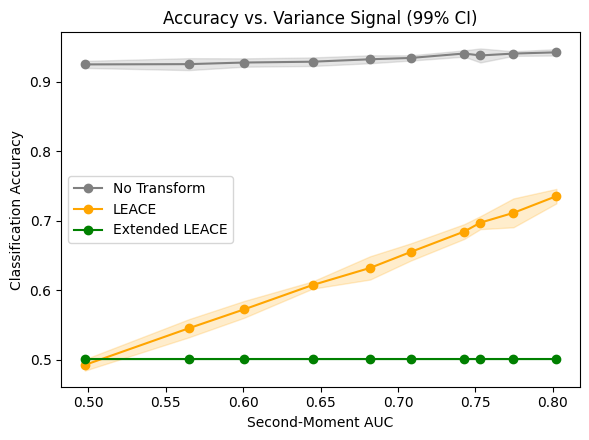
\includegraphics[width=0.6\linewidth]{accuracy_vs_auc.png}
    \caption{Classification Accuracy vs. AUC of Variance-Based Signal. Shaded regions denote 99\% confidence intervals over cross-validation folds.}
    \label{fig:acc_auc}
\end{figure*}
As shown in Figure~\ref{fig:acc_auc}, the classification accuracy is almost perfect as expected since the data is generated using that the dependency of $Z$ on $X$ is in the first or second-moment, Confirming that the classifiers exploit the second-moment differences between the classes.
\newline \newline
The LEACE-transformed representation shows that if only dependencies are in the first moment the classifiers after transformation has around a 50\% chance of predicting accurate which means it is close to "random guessing" for the classifier. But, when the second-moment AUC is increasing the classifier predicting accuracy after the LEACE transformation is also increasing. This is as expected since LEACE only aligns the first-moments but leaves the second-moment structure as it is.
\newline \newline
After the proposed extended LEACE transformation when almost all the dependencies are in the first-moment of the data, the classifier after transformation has exactly the same percentage of accuracy. which is inline with the theory since it uses the same first moment constraint. But in contrast of the LEACE framework, it stays around 50\% accuracy even when almost all the dependencies are in the second-moment of the data. Which means it consistently achieves near-random classification accuracy regardless of the second-moment strength, indicating that both linear and second-moment dependencies about $Z$ have been effectively removed with 99\% confidence \footnote{All reported metrics are averaged over 5-
fold cross-validation. For each measurement, the reported sample mean and 99\% confidence intervals are based on empirical standard errors.}.

\subsection{Distortion V.s. Second-Moment Signal Strength}
\begin{figure*}[t]
    \centering
    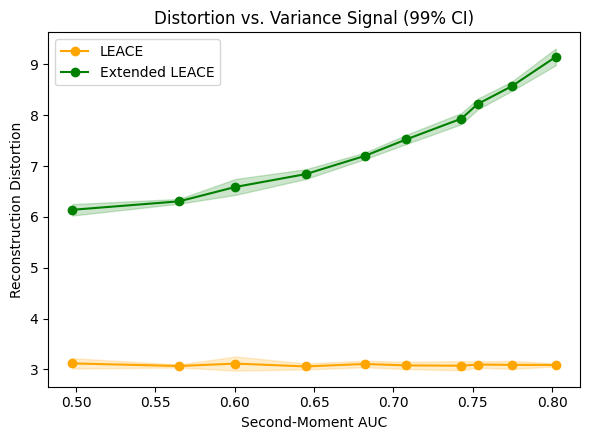
\includegraphics[width=0.6\linewidth]{distortion_vs_auc.png}
    \caption{Distortion vs. AUC of Variance-Based Signal. Shaded regions denote 99\% confidence intervals over cross-validation folds.}
    \label{fig:dist_auc}
\end{figure*}
Also the reconstruction distortion for both LEACE and the extension is evaluated. As shown in  Figure~\ref{fig:dist_auc}, The LEACE transformation shows low distortion across all strengths of second-moment dependencies, which is as expected since it only removes the first-moment dependencies of $Z$.
\newline \newline
The extended transformation exhibits a higher distortion even when all the dependencies of $Z$ are in the first-moment of the data, which is expected since it also changes the data in the second-moment of the class-conditional data. It also shows that when the second-moment dependency increases, the distortion also increases. Which shows us a trade-off between fairness and reconstruction distortion.
\newline \newline
These results support the theoretical motivation for second-moment matching and demonstrate the practical value of our closed-form extension to the LEACE framework.
\section{Conclusion}
While the LEACE (LEAst-squares Concept Erasure) framework of \cite{Belrose2023} effectively removes any linear correlations between the data and a sensitive attribute (e.g., gender or race) via first-moment matching, it does not account for dependencies in the second-moment of class-conditional data. As demonstrated in recent literature, such second-order dependencies can still be exploited by models to learn sensitive class relations.
\newline \newline
This study proposed an extension to the LEACE framework, aimed at addressing this limitation by matching both the first- and second-moment of the class-conditional distributions.
\newline \newline
The resulting transformation preserves much of the original representation while ensuring that the sensitive attribute can not be inferred by models relying on the first- or second-order statistics.
\newline \newline
Empirical evaluation confirms that the extension effectively removes second-moment dependencies. By using a Monte Carlo simulation, our method consistently removes inferences with the sensitive attribute in the first- and second-moment of the class-conditional data.
\newline \newline
Compared to LEACE, this method introduces more distortion but achieves significantly stronger fairness guarantees under both linear and quadratic classifiers.

\section{Discussion}
However, several limitations remain, First, this framework is not proven to be \emph{the} unique minimizer, hence there is a possibility that there this framework can be improved in its distortion. Second, it is still limited to second-order dependencies and does not remove higher-order dependencies or nonlinear dependencies in general. Finally, while the whitening step simplifies the derivation, it may introduces some noise in directions with small variance.
\newline \newline
Future research could extend on this study trying to find or proof the unique minimizer in distortion while matching both moments, or extend this by including higher moments matching in the constraints while minimizing the distortion. In addition, applying this framework to real-world datasets, such as credit risk models, would help showing its practical impact and robustness.

\newpage
%%%%%%%%%%%%%%%%%%%%%%%%%%%%%%%%%%%%%%%%%%%%%%
%% Bibliography:                            %%
%%%%%%%%%%%%%%%%%%%%%%%%%%%%%%%%%%%%%%%%%%%%%%
%% IMPORTANT: References in the bibliography should be complete, 
%% including the first and last names, and date of publication.

%% If your bibliography is in bibtex format, uncomment commands:
%\bibliographystyle{ecta-fullname} % Style BST file
%\bibliography{bibliography}  % Bibliography file (usually '*.bib')

%% Or include bibliography directly:

\bibliographystyle{ecta-fullname}
\bibliography{mainbib}
\end{multicols}{2}
\newpage
\begin{appendix}
\section{Derivation Framework}
%\subsection{Whitening Transformation} \label{Whitening Transformation}
\subsection{Proposition 1} \label{Proposition 1}
We derive the affine transformation
$$
s(\mathbf{x}) := \mathbf{P}\mathbf{x} + \mathbf{b}, \quad \text{where} \quad 
\mathbf{P} := \mathbf{W}^{-1} (\mathbf{I} - \mathbf{U}_W \mathbf{U}_W^\top) \mathbf{W}, \quad 
\mathbf{b} := (\mathbf{I} - \mathbf{P}) \boldsymbol{\mu},
$$
used to enforce statistical parity by eliminating both first- and second-moment disparities across groups.

Let $\mathbf{x} \in \mathbb{R}^d$, $\mathbf{P} \in \mathbb{R}^{d \times d}$, $\mathbf{b} \in \mathbb{R}^d$, $\mathbf{z} \in \{0,1\}^k$. 
Let $\boldsymbol{\mu}^{(z)} := \mathbb{E}[\mathbf{x} \mid \mathbf{z}=z]$ and covariances $\boldsymbol{\Sigma}^{(z)} := \operatorname{Cov}(\mathbf{x} \mid \mathbf{z}=z)$ for $z \in \{0,1\}$. We define the mean and covariance differences:
$$
\boldsymbol{\Delta}_{\mu} := \boldsymbol{\mu}^{(1)} - \boldsymbol{\mu}^{(0)}, \quad \boldsymbol{\Delta}_{\Sigma} := \boldsymbol{\Sigma}^{(1)} - \boldsymbol{\Sigma}^{(0)},
$$
and the pooled covariance:
$$
\boldsymbol{\Sigma} := \tfrac{1}{2}(\boldsymbol{\Sigma}^{(0)} + \boldsymbol{\Sigma}^{(1)}), \quad \boldsymbol{\mu} := \tfrac{1}{2}(\boldsymbol{\mu}^{(0)} + \boldsymbol{\mu}^{(1)}).
$$

We seek a transformation $s(\mathbf{x}) = \mathbf{P}\mathbf{x} + \mathbf{b}$ where $\mathbf{\mathbf{P}}$ minimizes $\mathbb{E}\left[ \| \mathbf{P}\mathbf{x} - \mathbf{x} \|^2_{2} \right]$ while ensuring statistical parity by enforcing:
\begin{align*}
    &\text{Cov}(\mathbf{P}\mathbf{x},\mathbf{z}) = \mathbf{0} \\ &\Rightarrow \mathbb{E}[s(\mathbf{x}) \mid \mathbf{z} = 1] = \mathbb{E}[s(\mathbf{x}) \mid \mathbf{z} = 0]  \\ &\Leftrightarrow \mathbb{E}[\mathbf{P}\mathbf{x} + \mathbf{b} \mid \mathbf{z}=1]=\mathbb{E}[\mathbf{P}\mathbf{x} + \mathbf{b} \mid \mathbf{z}=0] \\ &\Leftrightarrow \mathbf{\mathbf{P}}\boldsymbol{\mu}^{(1)} = \mathbf{\mathbf{P}}\boldsymbol{\mu}^{(0)} \\ &\Leftrightarrow \mathbf{\mathbf{P}}(\boldsymbol{\mu}^{(1)} - \boldsymbol{\mu}^{(0)}) = \mathbf{0} \\ &\Rightarrow \mathbf{\mathbf{P}}\boldsymbol{\Delta}_{\mu} = \mathbf{0}
\end{align*}
\begin{align*}
    &\boldsymbol{\Sigma}^{(1)} = \boldsymbol{\Sigma}^{(0)}\\ 
    &\Rightarrow \mathbb{E}[s(\mathbf{x})s(\mathbf{x})^{\top} \mid \mathbf{z} = 1] = \mathbb{E}[s(\mathbf{x})s(\mathbf{x})^{\top} \mid \mathbf{z} = 0 ] \\ 
    &\Leftrightarrow \mathbb{E}[(\mathbf{P}\mathbf{x}+\mathbf{b})(\mathbf{P}\mathbf{x}+\mathbf{b})^{\top} \mid \mathbf{z} = 1] = \mathbb{E}[(\mathbf{P}\mathbf{x}+\mathbf{b})(\mathbf{P}\mathbf{x}+\mathbf{b})^{\top} \mid \mathbf{z} = 0] \\ 
    &\Leftrightarrow \mathbb{E}[\mathbf{P}\mathbf{x}\mathbf{x}^{\top}\mathbf{\mathbf{P}}^{\top} + 2\mathbf{P}\mathbf{x}\mathbf{b}^{\top} + \mathbf{b}\mathbf{b}^{\top} \mid \mathbf{z} = 1] = \mathbb{E}[\mathbf{P}\mathbf{x}\mathbf{x}^{\top}\mathbf{\mathbf{P}}^{\top} + 2\mathbf{P}\mathbf{x}\mathbf{b}^{\top} + \mathbf{b}\mathbf{b}^{\top} \mid \mathbf{z} = 0] \\ 
    &\Leftrightarrow \mathbf{\mathbf{P}}\mathbb{E}[\mathbf{x}\mathbf{x}^{\top} \mid \mathbf{z} =1]\mathbf{\mathbf{P}}^{\top} + 2\mathbf{P}\mathbb{E}[\mathbf{x} \mid \mathbf{z} = 0]\mathbf{b}^{\top} = \mathbf{\mathbf{P}}\mathbb{E}[\mathbf{x}\mathbf{x}^{\top} \mid \mathbf{z} =0]\mathbf{\mathbf{P}}^{\top} + 2\mathbf{P}\mathbb{E}[\mathbf{x} \mid \mathbf{z} = 0]\mathbf{b}^{\top} \\ 
    &\Leftrightarrow \mathbf{\mathbf{P}}\boldsymbol{\Sigma}^{(1)}\mathbf{\mathbf{P}}^{\top} = \mathbf{\mathbf{P}}\boldsymbol{\Sigma}^{(0)}\mathbf{\mathbf{P}}^{\top} \\ 
    &\Leftrightarrow \mathbf{\mathbf{P}}(\boldsymbol{\Sigma}^{(1)} - \boldsymbol{\Sigma}^{(0)})\mathbf{\mathbf{P}}^{\top} = \mathbf{0}  \\ 
    &\Rightarrow \mathbf{\mathbf{P}}\Delta_{\Sigma}\mathbf{\mathbf{P}}^{\top}
\end{align*}

We solve the objective as a constrained minimization:
$$
\min_{\mathbf{\mathbf{P}}, \mathbf{b}} \ \mathbb{E} \left[ \tfrac{1}{2} \|\mathbf{x} - \mathbf{P}\mathbf{x} - \mathbf{b}\|^2 \right]
\quad \text{subject to} \quad
\mathbf{\mathbf{P}} \boldsymbol{\Delta}_{\mu} = \mathbf{0}, \quad \mathbf{\mathbf{P}} \boldsymbol{\Delta}_{\Sigma} \mathbf{\mathbf{P}}^\top = \mathbf{0}.
$$
Introducing a vector Lagrange multiplier $\boldsymbol{\lambda} \in \mathbb{R}^d$ and a matrix multiplier $\boldsymbol{\Lambda} \in \mathbb{R}^{d \times d}$, the Lagrangian becomes:
\begin{align*}
    &\mathcal{L}(\mathbf{\mathbf{P}}, \mathbf{b}, \boldsymbol{\lambda}, \boldsymbol{\Lambda}) = \mathbb{E}\left[\frac{1}{2}\|\mathbf{x} - \mathbf{P}\mathbf{x} - \mathbf{b}\|^{2}_{2}\right] + \boldsymbol{\lambda}^\top \mathbf{\mathbf{P}} \boldsymbol{\Delta}_{\mu} + \mathrm{Tr}(\boldsymbol{\Lambda}^\top \mathbf{\mathbf{P}} \boldsymbol{\Delta}_{\Sigma} \mathbf{\mathbf{P}}^\top) \\
    \frac{\partial \mathcal{L}}{\partial \mathbf{\mathbf{P}}} = \mathbf{0} &\Rightarrow -\mathbb{E}[\mathbf{x}\mathbf{x}^{\top}] + \mathbb{E}[\mathbf{x}]\mathbf{b}^{\top} + \mathbf{\mathbf{P}}\mathbb{E}[\mathbf{x}\mathbf{x}^{\top}] + \boldsymbol{\lambda}^{\top}\boldsymbol{\Delta}_{\mu} + (\boldsymbol{\Lambda}^{\top}+\boldsymbol{\Lambda})\mathbf{\mathbf{P}}\boldsymbol{\Delta}_{\Sigma} = \mathbf{0} \\
    &\Leftrightarrow (\mathbf{\mathbf{P}}-\mathbf{I})\boldsymbol{\Sigma} + \boldsymbol{\mu} \mathbf{b}^{\top} + \boldsymbol{\lambda}^{\top}\boldsymbol{\Delta}_{\mu} + (\boldsymbol{\Lambda}^{\top}+\boldsymbol{\Lambda})\mathbf{\mathbf{P}}\boldsymbol{\Delta}_{\Sigma} = \mathbf{0} \\
    \frac{\partial \mathcal{L}}{\partial \boldsymbol{\lambda}} = \mathbf{0} &\Rightarrow \mathbf{\mathbf{P}} \boldsymbol{\Delta}_{\Sigma} = \mathbf{0} \\
    \frac{\partial \mathcal{L}}{\partial \boldsymbol{\Lambda}} = \mathbf{0} &\Rightarrow \mathbf{\mathbf{P}}\boldsymbol{\Delta}_{\Sigma}\mathbf{\mathbf{P}}^{\top} = \mathbf{0} \\
    \frac{\partial \mathcal{L}}{\partial \mathbf{b}} = \mathbf{0} &\Rightarrow \mathbf{\mathbf{P}}\mathbb{E}[\mathbf{x}] - \mathbb{E}[\mathbf{x}] + \mathbf{b} = \mathbf{0} \Rightarrow \mathbf{b}^{*} = (\mathbf{I} - \mathbf{\mathbf{P}})\boldsymbol{\mu}
\end{align*}

We aim to define a subspace $V \subseteq \mathbb{R}^d$ that captures all linear directions in the data responsible for statistical dependence on the sensitive attribute $\mathbf{z}$. In the whitened space, these directions are defined as:

\begin{enumerate}
    \item The group mean difference:
    $$
    \tilde{\boldsymbol{\Delta}}_{\mu} := \mathbf{W} \boldsymbol{\Delta}_{\mu} = \mathbf{W}(\boldsymbol{\mu}^{(1)} - \boldsymbol{\mu}^{(0)}),
    $$

    \item The group covariance difference:
    $$
    \tilde{\boldsymbol{\Delta}}_{\Sigma} := \mathbf{W} \boldsymbol{\Delta}_{\Sigma} \mathbf{W}^\top = \mathbf{W}(\boldsymbol{\Sigma}^{(1)} - \boldsymbol{\Sigma}^{(0)})\mathbf{W}^\top.
    $$
\end{enumerate}

\paragraph{Spectral Characterization of $\tilde{\boldsymbol{\Delta}}_{\Sigma}$.}

Let $\tilde{\boldsymbol{\Delta}}_{\Sigma}$ have the eigenvalue decomposition:
$$
\tilde{\boldsymbol{\Delta}}_{\Sigma} = \mathbf{Q} \mathbf{\mathbf{D}}_{\Delta} \mathbf{Q}^\top,
$$
where $\mathbf{\mathbf{D}}_{\Delta}$ is a diagonal matrix of real eigenvalues, and $\mathbf{Q}$ contains the corresponding orthonormal eigenvectors.
\newline \newline
The image of $\tilde{\boldsymbol{\Delta}}_{\Sigma}$ is given by:
$$
\operatorname{Im}(\tilde{\boldsymbol{\Delta}}_{\Sigma}) = \mathrm{span}\left\{ q_i : (D_\Delta)_{ii} \neq 0 \right\},
$$
In other words, the subspace spanned by eigenvectors corresponding to nonzero eigenvalues.

\paragraph{Construction of Subspace $V$.}

We define the subspace:
$$
V := \operatorname{span} \left( \tilde{\boldsymbol{\Delta}}_{\mu}, \operatorname{Im}(\tilde{\boldsymbol{\Delta}}_{\Sigma}) \right),
$$
which captures both first- and second-order statistical differences across groups.
\newline \newline
We then compute an orthonormal basis $\mathbf{\mathbf{U}}_W \in \mathbb{R}^{d \times k}$ of $V$ (with $k \leq d$), via combining $\tilde{\boldsymbol{\Delta}}_{\mu}$ with the eigenvectors of $\tilde{\boldsymbol{\Delta}}_{\Sigma}$ associated with nonzero eigenvalues and Applying Gram-Schmidt orthonormalization.
\newline\newline
Let $\boldsymbol{\Sigma} = \mathbf{U} \mathbf{D} \mathbf{U}^\top$ be the eigendecomposition of the pooled covariance matrix, and define the whitening and de-whitening transforms as:
$$
\mathbf{W} := \mathbf{D}^{-1/2} \mathbf{U}^\top, \qquad \mathbf{W}^{-1} := \mathbf{U} \mathbf{D}^{1/2}.
$$
The whitened variables are:
$$
\tilde{\mathbf{x}} := \mathbf{W} \mathbf{x}, \quad \tilde{\boldsymbol{\Delta}}_{\mu} := \mathbf{W} \boldsymbol{\Delta}_{\mu}, \quad \tilde{\boldsymbol{\Delta}}_{\Sigma} := \mathbf{W} \boldsymbol{\Delta}_{\Sigma} \mathbf{W}^\top,
$$
ensuring $\operatorname{Cov}(\tilde{\mathbf{x}}) = \mathbf{I}$.
\newline \newline
We define the orthogonal projection onto the complement of $V$ as:
$$
\tilde{\mathbf{\mathbf{P}}} := \mathbf{I} - \mathbf{U}_W \mathbf{U}_W^\top.
$$

Returning to the original space, we define the affine transformation:
\begin{align*}
\mathbf{\mathbf{P}} &:= \mathbf{W}^{-1} \tilde{\mathbf{\mathbf{P}}} \mathbf{W} = \mathbf{W}^{-1} (\mathbf{I} - \mathbf{U}_W \mathbf{U}_W^\top) \mathbf{W}, \\
\mathbf{b} &:= (\mathbf{I} - \mathbf{\mathbf{P}}) \boldsymbol{\mu},
\end{align*}
so that the final transformation is:
\begin{align*}
    s(\mathbf{x}) :=& \mathbf{W}^{-1} (\mathbf{I} - \mathbf{U}_W \mathbf{U}_W^\top) \mathbf{W}\mathbf{x} + (\mathbf{I} - \mathbf{W}^{-1} (\mathbf{I} - \mathbf{U}_W \mathbf{U}_W^\top) \mathbf{W}) \mu \\
    =& \mathbf{U} \mathbf{D}^{1/2} (\mathbf{I} - \mathbf{U}_W \mathbf{U}_W^\top)  \mathbf{D}^{-1/2} \mathbf{U}^\top \mathbf{x} + (\mathbf{I} - \mathbf{U} \mathbf{D}^{1/2} (\mathbf{I} - \mathbf{U}_W \mathbf{U}_W^\top)  \mathbf{D}^{-1/2} \mathbf{U}^\top ) \boldsymbol{\mu}
\end{align*}
This transformation satisfies:
$$
\mathbf{\mathbf{P}} \boldsymbol{\Delta}_{\mu} = \mathbf{0}, \quad \mathbf{\mathbf{P}} \boldsymbol{\Delta}_{\Sigma} \mathbf{\mathbf{P}}^\top = \mathbf{0}, \quad \mathbb{E}[s(\mathbf{x})] = \boldsymbol{\mu},
$$
\begin{comment}
\subsubsection{Uniqueness of the Minimizer}
\begin{enumerate}
    \item Strict convexity.
        Having that $b=(I-P)\mu$, the objective $$\frac{1}{2}\mathbb E\|X - s(X)\|_2^2 = \frac{1}{2}\mathrm{Tr}[(I-P)\Sigma(I-P)^\top]$$ is a strictly convex quadratic in the entries of $P$, since its Hessian in $P$ is $2(\Sigma\otimes I) \succ 0$.

    \item Affine constraints.
        Both $P\Delta\mu=0$ and $P\Delta\Sigma P^\top=0$ are linear (affine) equations in $P$.

    \item KKT implies uniqueness.
        A strictly convex objective over an affine feasible set has exactly one stationary (KKT) point, which is the global minimizer (cf.\ \cite[Thm.~4.2.1]{Boyd04}).  Since the above derivation finds a single $$(P^*,b^*)$$ satisfying KKT, it is the unique minimizer.
\end{enumerate}

ensuring alignment of first and second moments across groups while minimally changing the original data.
\end{comment}

\end{appendix}
\end{document}
